%234567890          1234567890          1234567890          1234567890
%         1234567890          1234567890          1234567890          1234567890
\documentclass[a4paper,11pt,twoside]{report}
\usepackage{dotss}
\usepackage{xr}
\usepackage{a4wide}
\usepackage{amsmath}
\usepackage{amssymb}

\begin{document}
\newcommand{\coursename}{Visualization (2IV35)}
\newcommand{\doctitle}{Practical assignment }
\newcommand{\docversion}{0.1}
\newcommand{\docdate}{\today}

\newcommand{\imagescalefactor}{0.40}

\dotsspreamble

\tableofcontents

\dotssdocument

\chapter{Introduction}
% Waar gaat het practicum over
\chapter{Overview}
% 'ontwerp' van de code
\chapter{Detailed description}
	\section{Skeleton compilation}
		\begin{figure}[h]
		\centering
		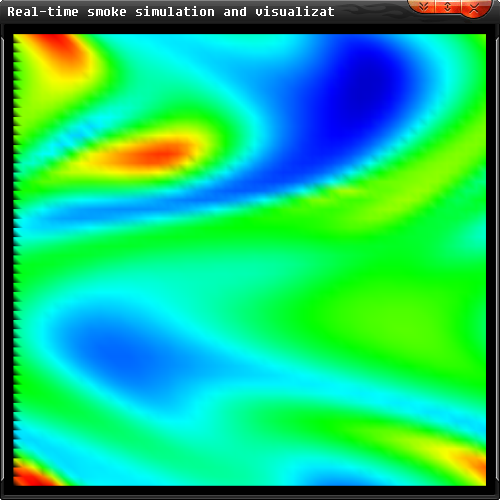
\includegraphics[scale=\imagescalefactor]{images/step1.png}
		\caption{The initial look of the progam}\label{fig:step1}
		\end{figure}
		\newpage
	\section{Color mapping}
		\begin{figure}[h]
		\centering
		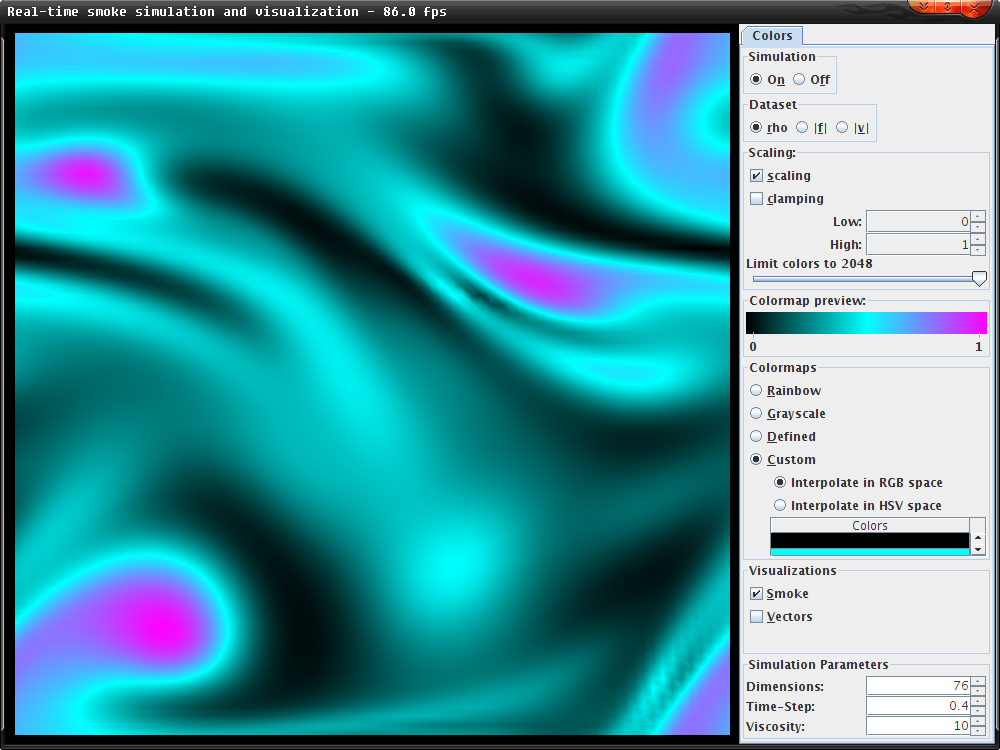
\includegraphics[scale=\imagescalefactor]{images/step2.png}
		\caption{First gui elements}\label{fig:step1}
		\end{figure}
		\newpage
	\section{Glyphs}
		\begin{figure}[h]
		\centering
		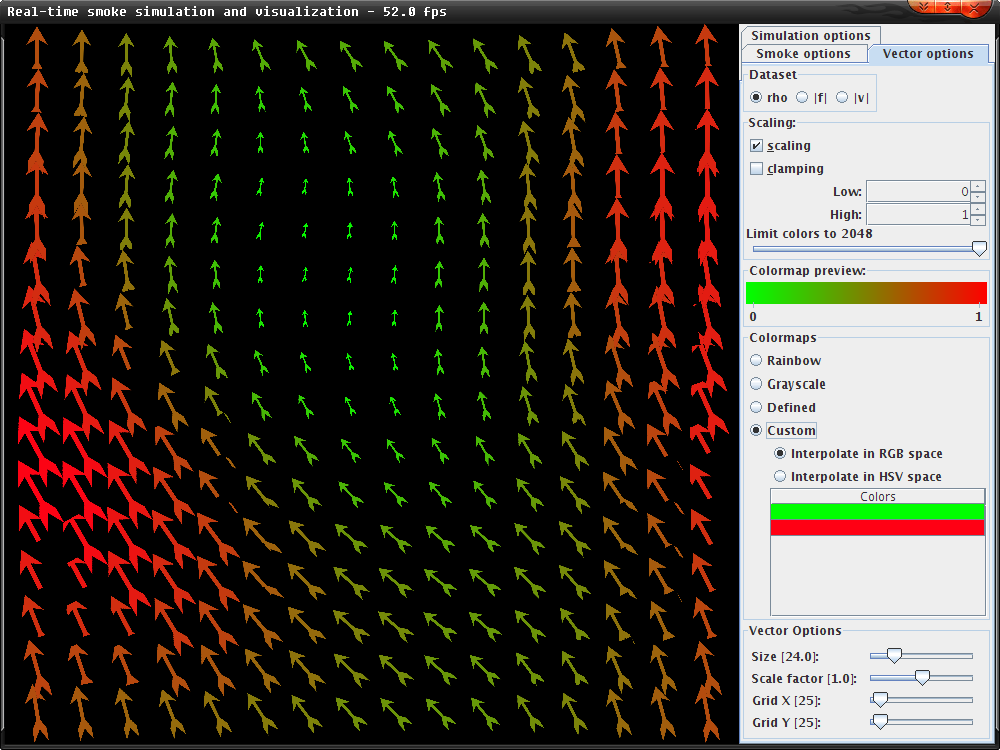
\includegraphics[scale=\imagescalefactor]{images/step3.png}
		\caption{Glyphs}\label{fig:step1}
		\end{figure}
		\newpage
	\section{Divergence}
		\begin{figure}[h]
		\centering
		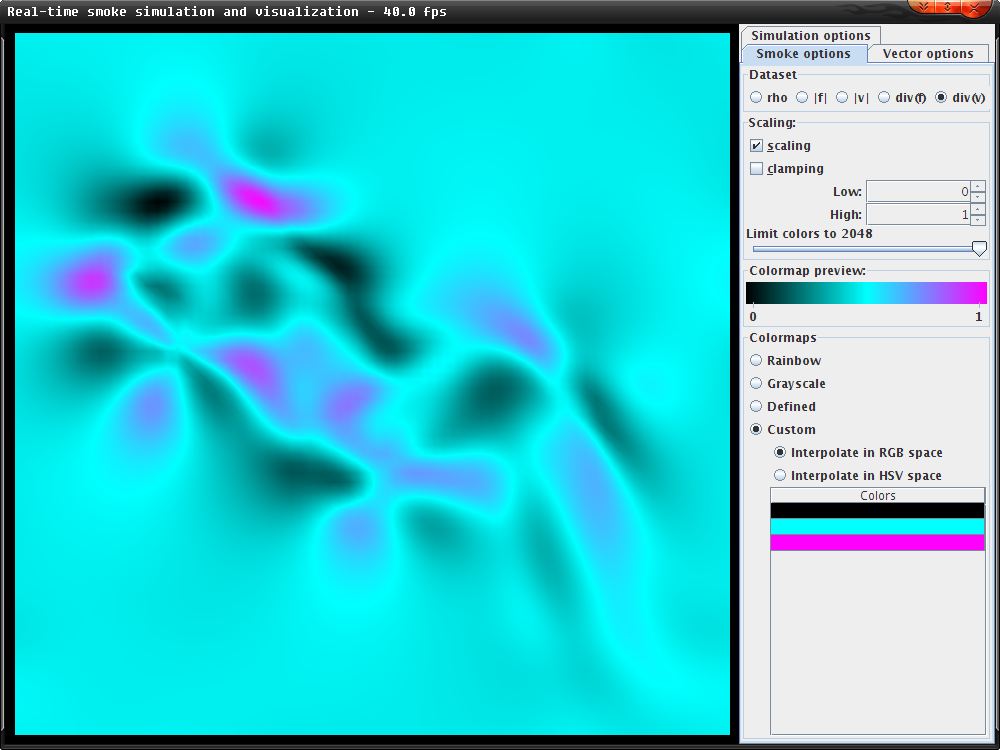
\includegraphics[scale=\imagescalefactor]{images/step4.png}
		\caption{Divergence}\label{fig:step1}
		\end{figure}
		\newpage
	\section{Isosurfaces (Isolines)}
		\begin{figure}[h]
		\centering
		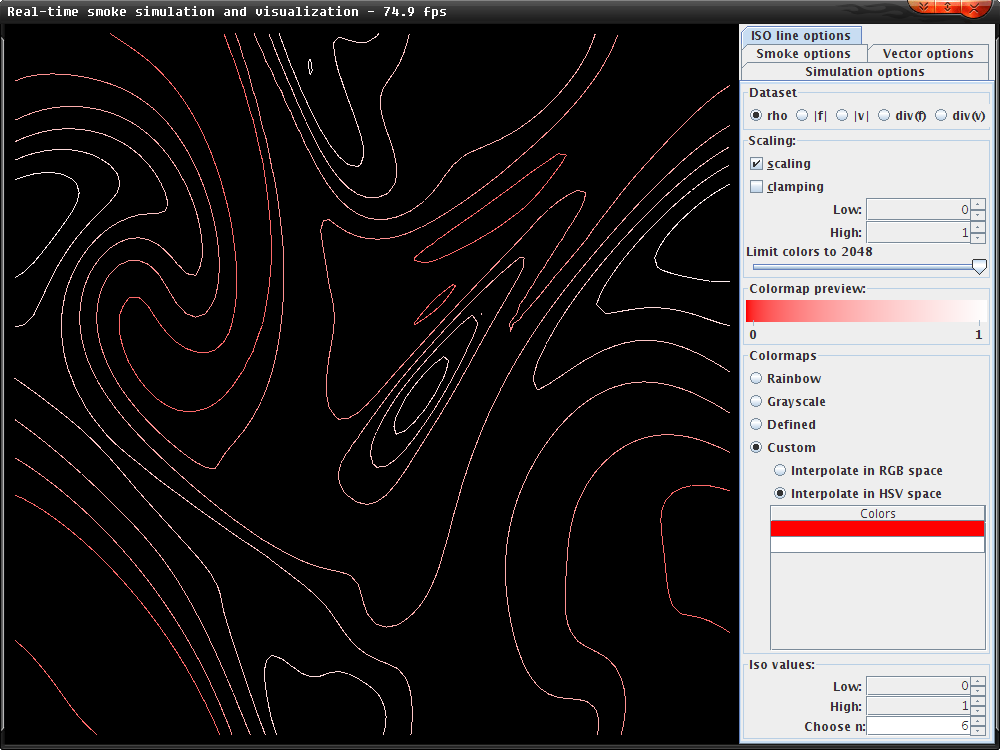
\includegraphics[scale=\imagescalefactor]{images/step5.png}
		\caption{Isolines}\label{fig:step1}
		\end{figure}
		\newpage
	\section{Height plots}
		\begin{figure}[h]
		\centering
		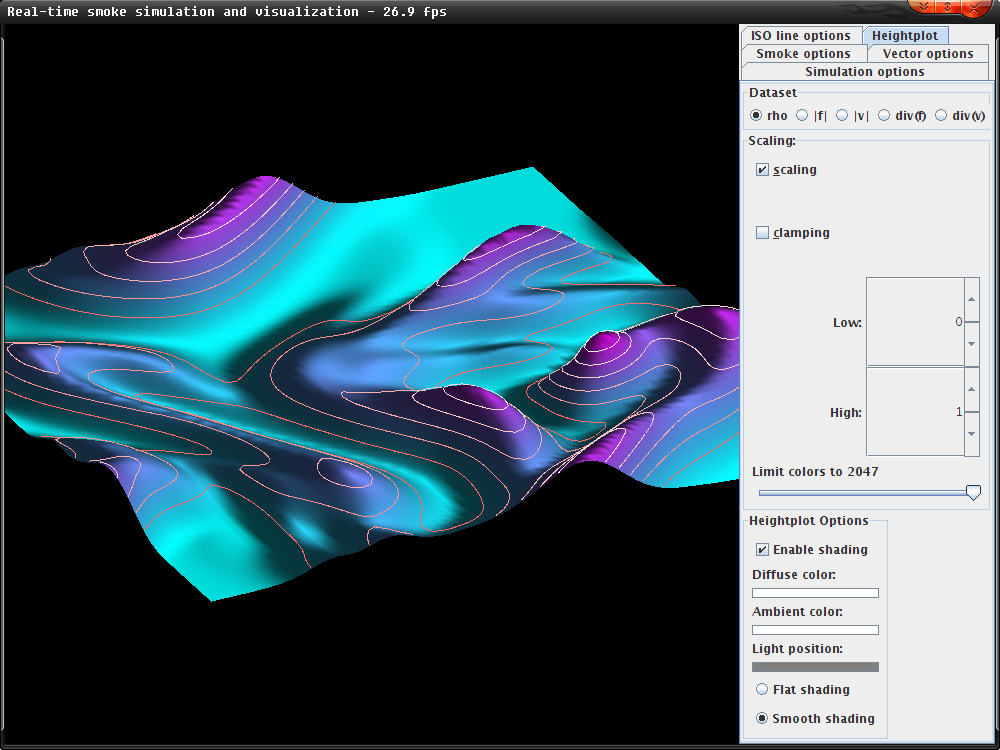
\includegraphics[scale=\imagescalefactor]{images/step6.png}
		\caption{The heightplot}\label{fig:step1}
		\end{figure}
		\newpage
	\section{Stream tubes}
\chapter{Conclusion}
% klein stukje slap gezever
\end{document}
